\documentclass[conference]{IEEEtran}
\IEEEoverridecommandlockouts

\usepackage[utf8]{inputenc}
\usepackage[T1]{fontenc}

\usepackage{CJKutf8}
\usepackage{datetime}
\usepackage{amsmath}
\usepackage{amssymb}
\usepackage{mathtools}
\usepackage{subcaption}
\usepackage{xcolor}
\usepackage{ulem}
\usepackage{hyperref}
\usepackage{graphicx}
\usepackage{cite}
\usepackage{multirow}
\usepackage{makecell}
\usepackage{url}

\graphicspath{{images/}}
\DeclareGraphicsExtensions{.pdf}

\begin{document}

\title{Ensuring Fairness with Transparent Auditing of Quantitative Bias in AI Systems\\
\thanks{Identify applicable funding agency here. If none, delete this.}
}

\author{\IEEEauthorblockN{1\textsuperscript{st} Given Name Surname}
\IEEEauthorblockA{\textit{dept. name of organization (of Aff.)} \\
\textit{name of organization (of Aff.)}\\
City, Country \\
email address or ORCID}
\and
\IEEEauthorblockN{2\textsuperscript{nd} Given Name Surname}
\IEEEauthorblockA{\textit{dept. name of organization (of Aff.)} \\
\textit{name of organization (of Aff.)}\\
City, Country \\
email address or ORCID}
}

\DeclarePairedDelimiter{\set}{\{}{\}}
\DeclarePairedDelimiter{\tuple}{(}{)}
\DeclarePairedDelimiter{\abs}{\lvert}{\rvert}

\renewcommand{\implies}{\rightarrow}

\newcommand{\db}{\mathcal{D}}
\newcommand{\model}{\mathcal{M}}
\newcommand{\priv}{P}
\newcommand{\pos}{\hat{P}}
\newcommand{\tru}{T}
\newcommand{\leg}{L}
\newcommand{\sco}{\hat{S}}

\newcommand{\bye}[1]{}

% \author{\IEEEauthorblockN{1\textsuperscript{st} Chih-Cheng Rex Yuan}
% \IEEEauthorblockA{\textit{Institute of Information Science} \\
% \textit{Academia Sinica}\\
% Taipei, Taiwan \\
% hello@rexyuan.com}
% \and
% \IEEEauthorblockN{2\textsuperscript{nd} Bow-Yaw Wang}
% \IEEEauthorblockA{\textit{Institute of Information Science} \\
% \textit{Academia Sinica}\\
% Taipei, Taiwan \\
% bywang@iis.sinica.edu.tw}
% }

\maketitle

\begin{abstract}
With the rapid advancement of AI, there is a growing trend to integrate AI into decision-making processes. However, AI systems may exhibit biases that lead decision makers to draw unfair conclusions. Notably, the COMPAS system used in the American justice system to evaluate recidivism was found to favor racial majority groups; specifically, it violates a fairness standard called equalized odds. Various measures have been proposed to assess AI fairness. We present a framework for auditing AI fairness, involving third-party auditors and AI system provider, and we have created a tool to facilitate systematic examination of AI systems. Inclusion of independent and trusted auditors is pivotal for objectivity and accountability; third parties are often further necessary for their specialized expertise in relevant domains. Auditors, equipped with our tool, can thoroughly review AI systems for bias and fairness violations. The tool is open-sourced and publicly available. Unlike traditional AI systems, we advocate a transparent white-box and statistics-based approach. It can be utilized by third party auditors, AI developers, or the general public for reference when judging the fairness criterion of AI systems.
\end{abstract}

\begin{IEEEkeywords}
AI, fairness, auditing
\end{IEEEkeywords}

\section{Introduction}
In recent years, the accelerating pace of artificial intelligence (AI) technologies have revolutionized numerous fields. In healthcare, AI-driven diagnostic systems streamline disease identification, while in finance, automated trading algorithms analyze market trends to execute optimal trades swiftly. This remarkable progress has reached diverse industries, sprouting out various applications for different purposes.

One of its most profound impact is how AI has transformed decision-making processes across sectors. By harnessing vast amounts of data and employing advanced algorithms, AI empowers organizations to make more informed and strategic decisions. From assessing job applicants to determining school admissions, AI-driven insights offer efficient and analytical advantages.

AI system, however, may be biased. Factors such as inherent biases in original data sets or flaws in algorithm designs could contribute to bias within AI systems. When left unchecked, the ramifications of such biases extend far beyond mere inaccuracies; it can lead to devastating consequences, such as amplifying systemic injustices, perpetuating group discrimination, and exacerbating societal inequalities.

Correctional Offender Management Profiling for Alternative Sanctions (COMPAS) is a tool for predicting recidivism---the tendency of criminals to reoffend. It is used in the criminal justice system in multiple states in the United States. In 2016, it was discovered in an investigation by the journalists at ProPublica that the COMPAS system is, in fact, unfair towards minority and disadvantaged groups.

Cases such as COMPAS underscore the critical importance of rigorously examining the fairness of AI systems by third parties. Fairness is fundementally a subjective social construct, heavily influenced by cultural context and deeply rooted in historical inequalities. However, there have been development in research leveraging statistical metrics to quantify fairness that provide transparent and objective insights.

By employing such mathematically rigorous methodologies, our research can offer a more deeper look into the fairness of AI systems, enabling third parties to make more informed and robust judgment. For example, it would reveal that the COMPAS system violates a fairness measure called equalized odds.

In addition to equalized odds, there are a number of fairness measures for AI systems. Our framework aims to help third parties apply these metrics and navigate complex datasets with ease, pinpointing instances of bias and discrimination.

With our tool, a third party such as ProPublica could clearly and easily demonstrates that COMPAS violates equalized odds according to their datasets. Our platform empowers organizations to conduct thorough assessments of AI fairness and uncover discrepancies in predictive models.

This functionality not only facilitates sound judgment but also fosters objectivity and transparency regarding AI systems, ultimately bolster the claim of fairness and justice in AI-enabled decision-making.

Our tool is written in Python and is offered as a Python package. It supports common datasets format such as csv. It is open-sourced and publicly available for downloads.

\section{Fairness Measures}
\label{sec:measures}
Fairness is about making sure the disadvantaged and unprivileged groups of individuals are treated equitably. However, there have been several interpretations of it proposed in the past. To have a constructive discussion on fairness, we must first have precise definitions of it. Pessach and Shmueli \cite{pessach2022review} formulated a number of fairness measures in an unified mathematical notation. We will base our framework on their formulation.

\subsection{Preliminaries}
For the following definition we will use $Y$ to denote the ground truth of an outcome; $\hat{Y}$ to denote the predicated result of an outcome; $Y = 1$ and $\hat{Y} = 1$ to denote them being accepted or positive. For example, let $Y$ be recidivism. Then $Y = 1$ means the case of an individual actually recidivating and $\hat{Y} = 0$ means the predication of an individual recidivating is negative. In addition, we use $V$ and $\hat{V}$ when the truth and the prediction isn't binary. For example, we denote COMPAS score by $\hat{V}$, which ranges from 1 to 10.

We denote by $S$ some protected attribute. Protected attributes are the characteristics of individuals that are, for example, legally or ethically, considered sensitive and warrant protection against discrimination and bias. We write $S = 1$ to represent the privileged group and $S \neq 1$ to represent the unprivileged group. For example, let $S$ be Caucasian. Then $S = 1$ represents the case of an individual's race being Caucasian and $S \neq 1$ vice versa.

We denote by $\epsilon$ some threshold that's used to limit the fairness measures.

\subsection{Disparate Impact}
In 1971 \cite{griggs1971}, the US spreme court ruled that it is illegal for hiring decisions to have  ``disparate impact'' by race, thus coining the term. It is taken as unintentional discrimination, as opposed to intentional discrimination, which is called ``disparate treatment''.

Legal cases involving disparate impact often refer to the ``80\% Rule'', advocated by the US Equal Employment Opportunity Commission \cite{eeoc1979}, where it requires the selection rate of a minority group is to be no less than 80\% of that of a majority group. Formally \cite{feldman2015certifying}, it is:

\[
    \frac{P[\hat{Y} = 1 | S \neq 1]}{P[\hat{Y} = 1 | S = 1]} \geq 1 - \epsilon
\]

In the case of 80\% rule, $\epsilon = 20\%$.

\subsection{Demographic Parity} %TODO: why cite this?
Demographic parity \cite{calders2010three}, also known as statistical parity, is similar to disparate impact but, instead of ratio, difference is taken. It is named so to suggest that each demographic group(such as race, gender, or age) should have equal representation or opportunity. Formally, it is:

\[
    \abs{P[\hat{Y} = 1 | S = 1] - P[\hat{Y} = 1 | S \neq 1]} \leq \epsilon
\]

\subsection{Conditional Statistical Parity}
Conditional statistical parity \cite{corbett2017algorithmic} is similar to demographic parity, but, in addition to protected attributes, it further takes into account some ``legitimate'' attributes that are \textit{legitimately} related to the case. For example, a legitimate attribute when considering future recidivism could be the number of prior crimes committed. Formally, it is:

\[
    \abs{P[\hat{Y} = 1 | S = 1, L = l] - P[\hat{Y} = 1 | S \neq 1, L = l]} \leq \epsilon
\]

where $L$ denotes the legitimate attributes.

\subsection{Overall Accuracy Equality}
Overall accuracy eqaulity \cite{berk2021fairness} is similar to demographic parity, but instead of the case of $\hat{Y} = 1$, it considers the case of $Y = \hat{Y}$; that is, the case where the prediction is accurate. Formally, it is:

\[
    \abs{P[Y = \hat{Y} | S = 1] - P[Y = \hat{Y} | S \neq 1]} \leq \epsilon
\]

\subsection{Mean Difference}
Mean difference \cite{vzliobaite2017measuring} considers the case of non-binary outcome, such as the score of COMPAS. It takes the expected value of the prediction. Formally, it is:

\[
    \abs{E[\hat{Y}|S = 1] - E[\hat{Y}|S \neq 1]} \leq \epsilon
\]

\subsection{Equalized Odds}
Equalized odds \cite{hardt2016equality} is similar to demogrphic parity, but it further takes into account the grouth truth. It consider the cases of true positive and false positive. It solves the downsides of a fully accurate classifier might be deemed unfair by measures that don't take ground truth into consideration. For example, consider a group $A$ that is predicated to recidivate and they do in fact always recidivate and a group $B$ that is predicated to recidivate but end up never recidivating. A fully accurate classifier will always predict $A$ to recidivate while $B$ to never recidivate, and this will violate demogrphic parity. By taking ground truth into account, equalized odds avoids these pitfalls. Formally, it is:

\begin{align*}
    \abs{P[\hat{Y} = 1 | S = 1, Y = 0] - P[\hat{Y} = 1 | S \neq 1, Y = 0]} & \leq \epsilon \\
    \abs{P[\hat{Y} = 1 | S = 1, Y = 1] - P[\hat{Y} = 1 | S \neq 1, Y = 1]} & \leq \epsilon
\end{align*}

\subsection{Equal Opportunity}
Equal opportunity \cite{hardt2016equality} is a relaxation of equalized odds by only considering the true positive case. It is named so because when outcome being positive is beneficial to the individual, as it is an opportunity, such as school acceptance, the fairness of the true positive case is much more important. Formally, it is:

\begin{align*}
    \abs{P[\hat{Y} = 1 | S = 1, Y = 1] - P[\hat{Y} = 1 | S \neq 1, Y = 1]} & \leq \epsilon
\end{align*}

\subsection{Predictive Equality}
Predictive equality \cite{corbett2017algorithmic} is also a relaxation of equalized odds by only considering the false positive case. It was formulated by considering positive outcome being detrimental to the individual, such as predicting future recidivism. Thus, only the false positive case is taken. Formally, it is:

\begin{align*}
    \abs{P[\hat{Y} = 1 | S = 1, Y = 0] - P[\hat{Y} = 1 | S \neq 1, Y = 0]} \leq \epsilon
\end{align*}

\subsection{Conditional Use Accuracy Equality}
Conditional use accuracy equality \cite{berk2021fairness} is similar to equalized odds, but instead of conditioning on the ground truth, it conditions on the prediction and calculated the probability of the ground truth. It can be seem as checking the prediction accuracy across groups, thus the name. It further requires the measure on the case of positive predictive values is less than that of the negative predictive values. Formally, it is:

\begin{align*}
    \abs{P[Y = 1 | S = 1, \hat{Y} = 1] & - P[Y = 1 | S \neq 1, \hat{Y} = 1]} && \leq \epsilon \\
    & \rotatebox{90}{>} && \\
    \abs{P[Y = 0 | S = 1, \hat{Y} = 0] & - P[Y = 0 | S \neq 1, \hat{Y} = 0]} && \leq \epsilon
\end{align*}

\subsection{Predictive Parity}
Predictive parity \cite{chouldechova2017fair} is a relaxation of conditional use accuracy equality by only considering the positive predictive value case. Like predictive equality, it was formulated by considering positive outcome being detrimental to the individual. Thus, only the positive predictive value case is taken. Formally, it is:

\begin{align*}
    \abs{P[Y = 1 | S = 1, \hat{Y} = 1] - P[Y = 1 | S \neq 1, \hat{Y} = 1]} \leq \epsilon
\end{align*}

\subsection{Equal Calibration}
Equal calibration \cite{chouldechova2017fair} is similar to equal opportunity, but instead of having a binary $\hat{Y}$, it is conditioned on the range of the predicted value $\hat{V}$. For example, this could be conditioned on the highest COMPAS score $\hat{V} = 10$. Calibration is a concept of having fair score function \cite{fraenkel2020fairness}. Formally, it is:

\begin{align*}
    \abs{P[Y = 1 | S = 1, \hat{V} = v] - P[Y = 1 | S \neq 1, \hat{V} = v]} \leq \epsilon
\end{align*}

\subsection{Positive Balance}
Positive balance \cite{kleinberg2016inherent} is similar to equal opportunity, but instead of taking the difference of probability of binary prediction $\hat{Y}$, it takes the difference of the expected value of the score $\hat{V}$. Formally, it is:

\begin{align*}
    \abs{E[\hat{V} | Y = 1, S = 1] - E[\hat{V} | Y = 1, S \neq 1]} \leq \epsilon
\end{align*}

\subsection{Negative Balance}
Negative balance \cite{kleinberg2016inherent} is like positive balance except it conditions on the case of $Y = 0$. Formally, it is:

\begin{align*}
    \abs{E[\hat{V} | Y = 0, S = 1] - E[\hat{V} | Y = 0, S \neq 1]} \leq \epsilon
\end{align*}

These fairness measures are compiled in Table~\ref{tab:measures}.

\begin{table*}[h]
    \centering
    % \resizebox{\textwidth}{!}{
    % \resizebox{\columnwidth}{!}{
    \begin{tabular}{|l|c|} % 'l' specifies left alignment for the first column
        \hline
        \textbf{Fairness Measure} & \textbf{Definition} \\
        \hline
Disparate Impact & $\frac{P[\hat{Y} = 1 | S \neq 1]}{P[\hat{Y} = 1 | S = 1]} \geq 1 - \epsilon$ \\
\hline
Demographic Parity & $\abs{P[\hat{Y} = 1 | S = 1] - P[\hat{Y} = 1 | S \neq 1]} \leq \epsilon$ \\
\hline
Conditional Statistical Parity & $\abs{P[\hat{Y} = 1 | S = 1, L = l] - P[\hat{Y} = 1 | S \neq 1, L = l]} \leq \epsilon$ \\
\hline
Overall Accuracy Eqaulity & $\abs{P[Y = \hat{Y} | S = 1] - P[Y = \hat{Y} | S \neq 1]} \leq \epsilon$ \\
\hline
Mean Difference & $\abs{E[\hat{Y}|S = 1] - E[\hat{Y}|S \neq 1]} \leq \epsilon$ \\
\hline
\multirow{2}{*}{Equalized Odds} & $\abs{P[\hat{Y} = 1 | S = 1, Y = 0] - P[\hat{Y} = 1 | S \neq 1, Y = 0]} \leq \epsilon$ \\
\cline{2-2}
                                & $\abs{P[\hat{Y} = 1 | S = 1, Y = 1] - P[\hat{Y} = 1 | S \neq 1, Y = 1]} \leq \epsilon$ \\
\hline
Equal Opportunity & $\abs{P[\hat{Y} = 1 | S = 1, Y = 1] - P[\hat{Y} = 1 | S \neq 1, Y = 1]} \leq \epsilon$ \\
\hline
Predictive Equality & $\abs{P[\hat{Y} = 1 | S = 1, Y = 0] - P[\hat{Y} = 1 | S \neq 1, Y = 0]} \leq \epsilon$ \\
\hline
\multirow{2}{*}{Conditional Use Accuracy Equality} & $\abs{P[Y = 1 | S = 1, \hat{Y} = 1] - P[Y = 1 | S \neq 1, \hat{Y} = 1]} \leq \epsilon$ \\
\cline{2-2}
                                 & $\abs{P[Y = 0 | S = 1, \hat{Y} = 0] - P[Y = 0 | S \neq 1, \hat{Y} = 0]} \leq \epsilon$ \\
\hline
Predictive Parity & $\abs{P[Y = 1 | S = 1, \hat{Y} = 1] - P[Y = 1 | S \neq 1, \hat{Y} = 1]} \leq \epsilon$ \\
\hline
Equal Calibration & $\abs{P[Y = 1 | S = 1, \hat{V} = v] - P[Y = 1 | S \neq 1, \hat{V} = v]} \leq \epsilon$ \\
\hline
Positive Balance & $\abs{E[\hat{V} | Y = 1, S = 1] - E[\hat{V} | Y = 1, S \neq 1]} \leq \epsilon$ \\
\hline
Negative Balance & $\abs{E[\hat{V} | Y = 0, S = 1] - E[\hat{V} | Y = 0, S \neq 1]} \leq \epsilon$ \\
\hline
    \end{tabular}
    % }
    \caption{Fairness measures.}
    \label{tab:measures}
\end{table*}

\section{Auditing Framework}
\label{sec:framework}
Per the review by Pessach and Shmueli \cite{pessach2022review}, we designed an auditing framework for calculating the various fairness measure. We offer two versions of fairness checkers: one for when the prediction positive results are readily available in csv input and one for when a model is provided. In most auditing cases the model version is preferred because csv result can be easily fabricated.

\subsection{Preliminaries}
Let $\db = \set{r_1, r_2, ...}$ be a database containing rows of data. Each row $r_i : \mathtt{str} \implies \mathtt{str}$ is a lookup table or dictionary. For example, $r_n(\text{``sex''}) = \text{``Female''}$ means $r_n$'s sex is female.

A model $\model : (\mathtt{str} \implies \mathtt{str}) \implies \alpha$ takes a row and returns the model's prediction result of some type $\alpha$.

A privileged predicate $\priv : (\mathtt{str} \implies \mathtt{str}) \implies \mathtt{bool}$ takes a row and determines if it belongs to the privileged group. For example, $\priv(r_i) := r_i(\text{``race''}) == \text{``Caucasian''}$ means the privileged group is those with race being Caucasian.

A positive predicate of rows $\pos : (\mathtt{str} \implies \mathtt{str}) \implies \mathtt{bool}$ takes a row and determines if its prediction is positive. For example, $\pos(r_i) := \mathtt{int}(r_i(\text{``score''})) > \text{``7''}$ means a row's prediction is positive if its score is greater than 7. A positive predicate of model results $\pos : \alpha \implies \mathtt{bool}$ takes a model's result and determines if it is positive. In the simplest case, the model returns a $\mathtt{bool}$, and the positive predicate can just be the idnetity function.

A ground truth predicate $\tru : (\mathtt{str} \implies \mathtt{str}) \implies \mathtt{bool}$ takes a row and gives the ground truth of the result.

A legitimate predicate $\leg : \alpha_i^n \implies (\mathtt{str} \implies \mathtt{str}) \implies \mathtt{bool}$, and similarly a score predicate $\sco : \alpha_i^n \implies (\mathtt{str} \implies \mathtt{str}) \implies \mathtt{bool}$, takes $n$ parameters and returns a row predicate. For example, $\sco(u, l)(r_i) := l < \mathtt{int}(r_i(\text{``score''})) < u$ first takes two parameters $u,l$ as upper bound and lower bound, and then decides if $r_i$'s prediction score is between them.

\subsection{Definitions}
We abstracted the idea of privileged groups and positive prediction as predicates to maximizes flexibility. With the proper predicates, any model output can be used; even prose-like response of generative models can be included given adequate predicates.

Given a datasets for auditing use, and given csv prediction results or the prediction model itself, we can calculate the fairness measures mentioned in Section~\ref{sec:measures} by:

\begin{align*}
\text{disparate\_impact} & (\epsilon, \model, \priv, \pos) \\
\text{demographic\_parity} & (\epsilon, \model, \priv, \pos) \\
\text{conditional\_statistical\_parity} & (\epsilon, \model, \priv, \pos, \leg, (args, ...)) \\
\text{overall\_accuracy\_eqaulity} & (\epsilon, \model, \priv, \pos, \tru) \\
\text{mean\_difference} & (\epsilon, \model, \priv, \pos) \\
\text{equalized\_odds} & (\epsilon, \model, \priv, \pos, \tru) \\
\text{equal\_opportunity} & (\epsilon, \model, \priv, \pos, \tru) \\
\text{predictive\_equality} & (\epsilon, \model, \priv, \pos, \tru) \\
\text{conditional\_use\_accuracy\_equality} & (\epsilon, \model, \priv, \pos, \tru) \\
\text{predictive\_parity} & (\epsilon, \model, \priv, \pos, \tru) \\
\text{equal\_calibration} & (\epsilon, \model, \priv, \sco, \tru, (args, ...)) \\
\text{positive\_balance} & (\epsilon, \model, \priv, \sco, \tru, (args, ...)) \\
\text{nagative\_balance} & (\epsilon, \model, \priv, \sco, \tru, (args, ...)) \\
\end{align*}

where $\mathcal{M}$ is optional if the input contains csv prediction results.

By calculating all of the available fairness measures, we provide the auditors a comprehensive perespective on the fairness performance of a model or dataset.

%TODO package url

\subsection{Application}
\label{sec:app}
In this section, we will apply the proposed framework to the ProPublica COMPAS dataset \cite{angwin2016machine,larson2016compas,larson2016propublica}.

Correctional Offender Management Profiling for Alternative Sanctions (COMPAS), developed by private company Northpointe (now Equivant), is a risk assessment software used in the American criminal justice system to evaluate the likelihood of a defendant reoffending. Defendants taking the COMPAS test are given a questionnaire about topics ranging from family history to personal ideology. The questionnaire are then fed to the software system along with a number of parameters like the defendants's age, and then the system will assign a risk score to them from 1-10, with 10 being the highest risk.

ProPublica is an American non-profit journalism organization focused on public interests. In 2016, they conduct an investigative report into the COMPAS system. They obtained the 2013-2014 COMPAS score data of over 10,000 defendants in Florida. They also obtained criminal records of these defendants through 2016 and compared if they actually recidivate or not. They only counted misdemeanors and felonies as recidivism but not less serious crimes such as infractions. In the study, they've found that black defendants are disproportionately scored higher than they actually are and white defendants are disproportionately scored lower than they actually are.

We shall start applying our framework. There's generally no formal guide on how to set $\epsilon$, so we will take the 80\% rule's case and set it as $\epsilon = 0.2$. For the $\epsilon$ of positive and negative balance, we shall use $\epsilon = 5$ as it is a reasonable choice.

Although this dataset scenario falls in the csv-as-input case in our framework, and thus the model $\model$ input isn't needed, we also trained two simple makeshift models using the dataset itself for demonstration that simply outputs binary $\mathtt{bool}$ prediction, ``will recidivate'' and ``will not recidivate'', and $\mathtt{int}$ risk score, $1$ to $10$. The model was trained by splitting the original dataset into 3 partitions: 60\% of the data was used for training; 20\% was used for validation; and the rest 20\% was used for calculating fairness measures. The accuracy of the binary model was about 60\% and the accuracy of the score model was about 25\%.

We will set the privileged predicate be to ``non-African-American'' so that the unprivileged group will be African-American to test if the African-American race is discriminated.
\[
    \priv(r_i) := r_i(\text{``race''}) \neq \text{``African-American''}
\]

As ProPublica referenced Northpointe's COMPAS Practitioners Guide and cited that ``medium''(5-7) and ``high''(8-10) categories of scores are considered to indicate a risk of recidivism, we set the positive predicate using the readily available category.
\[
    \pos(r_i) := r_i(\text{``score\_text''}) \in \set{\text{``Medium''},\text{``High''}}
\]
Alternatively, since we know the corresponding scores of the categories, we can define it using the scores themselves, too.
\[
    \pos(r_i) := 5 \leq \mathtt{int}(r_i(\text{``decile\_score''})) \leq 10
\]
On the other hand, when we're taking prediction input from our makeshift model, we simply return its result because it already gives a binary $\mathtt{bool}$ result: $\pos(r_i) := \model(r_i)$

For the ground truth predicate, the recidivism data is already present in the ProPublica dataset, so all we have to do is a simple lookup.
\[
    \tru(r_i) := r_i(\text{``two\_year\_recid''}) == \text{``1''}
\]

For the legitimate predicate, we may want to look at defendants with priors. Here we shall set $args = (0)$.
\[
    \leg(x)(r_i) := \mathtt{int}(r_i(\text{``priors\_count''})) > x
\]

For the score predicate, we may want to specifically look at risk scores between a specifically range. Here we shall set $args = (7,5)$.
\[
    \sco(u,l)(r_i) := l \leq \mathtt{int}(r_i(\text{``decile\_score''})) \leq u
\]

With these predicates defined, we can call the fairness measure functions and check if the measure hold or not. The results are compiled in Table~\ref{tab:results}. Since some of the fairness measures are equivalent, we write them in the same entry.

\begin{table}[h]
    \centering
    \begin{tabular}{|l|c|c|} % 'l' specifies left alignment for the first column
        \hline
        \textbf{Fairness Measure} & \textbf{Criterion} & \textbf{Pass} \\
        \hline
Disparate Impact & 1.81 > 0.8 & YES \\
\hline
Demographic Parity & 0.26 < 0.2 & NO \\
\hline
Conditional Statistical Parity & 0.25 < 0.2 & NO \\
\hline
Overall Accuracy Equality & 0.02 < 0.2 & YES \\
\hline
Mean Difference & 0.26 < 0.2 & NO \\
\hline
\makecell[l]{Equalized Odds (true positive) \\ Equal Opportunity} & 0.23 < 0.2 & NO \\
\hline
\makecell[l]{Equalized Odds (false positive) \\ Predictive Equality} & 0.22 < 0.2 & NO \\
\hline
\makecell[l]{Conditional Use Accuracy Equality (true positive) \\ Predictive Parity} & 0.06 < 0.2 & YES \\
\hline
Conditional Use Accuracy Equality (true negative) & 0.06 < 0.2 & YES \\
\hline
Equal Calibration & 0.03 < 0.2 & YES \\
\hline
Positive Balance & 1.6 < 5 & YES \\
\hline
Negative Balance & 1.4 < 5 & YES \\
\hline
    \end{tabular}
    \caption{Fairness measures of privileged group being Non-African-American.}
    \label{tab:results}
\end{table}

On first blush, it is curious that it satisfies disparate impact but not demographic parity. However, if we return to the definition, we'd see that disparate impact is meant to be used when being marked positive is an advantaged thing, while here in the COMPAS exmaple, being marked positive is a disadvantaged thing. Thus, henceforth we will exclude disparate impact from our analysis.

We can then immediately tell from the failing demographic parity, mean difference, and conditional statistical parity that COMPAS prediction results was unfair against African-American, even if we only consider the ones with prior crimes.

From the low overall accuracy equality and both conditional use accuracy equality criteria we can tell that the accuracy is similar across African-Americans and non-African-Americans.

From the failing equalized odds we can conclude that African-Americans are indeed treated unequally by the COMPAS system even after the ground truth is taken into account. This is the same conclusion reached by the ProPublica report.

From the low equal calibration we can tell that if we only consider the medium risk score, African-Americans aren't treated fairly.

Finally, if we look at positive and negative balance, we can see that they're of similar numbers. However, not much else can be said since the criterion $\epsilon = 5$ isn't actually justified.

Setting the privilege predicate to different races we can have a more comprehensive look over the dataset. We've checked the case of privilege predicate being Non-African-American, Non-Asian, Non-Caucasian, Non-Hispanic, and Non-Native-American. The results are shown in Figure~\ref{fig:compas}.

From the results we can first notice that the overall accuracy eqaulity is low for both the Non-Asian and Non-Native-American case. This can be explained by checking the original dataset which shows that there are only 32 and 18 rows, respectivly, in dataset of 7214 rows. Hence, the accuracy is naturally lower because of the small data size.

\begin{figure*}[h]
    \centering
    \begin{minipage}[b]{0.48\linewidth}
        \centering
        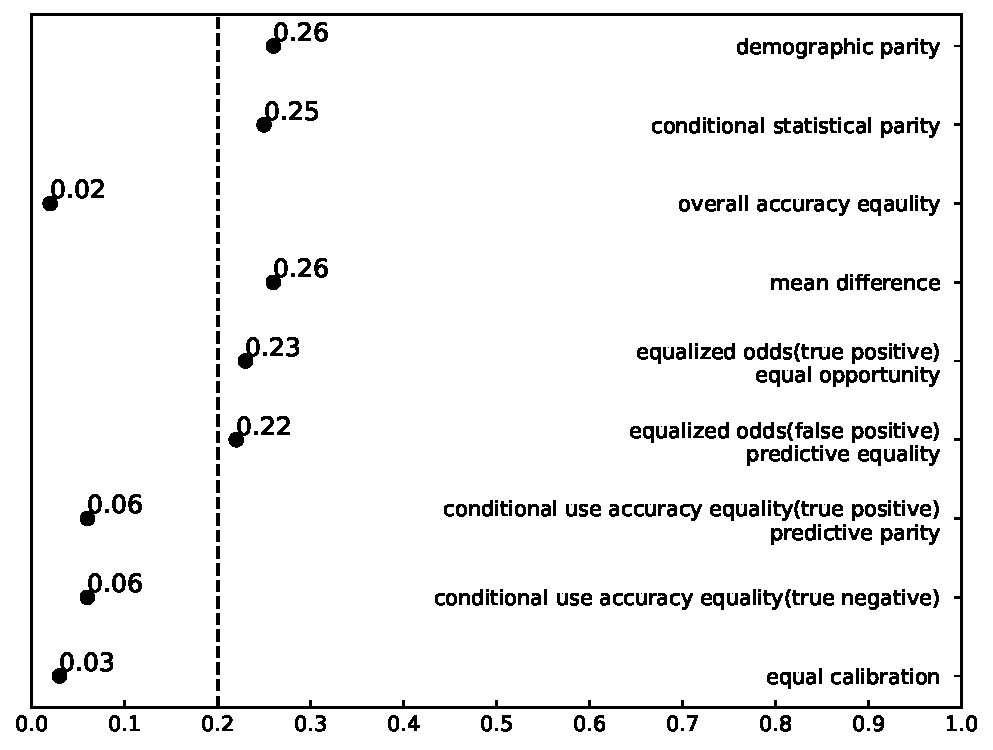
\includegraphics[width=\linewidth]{Non-African-American}
        \subcaption{Privileged Group: Non-African-American}\label{fig:1}
    \end{minipage}
    \hfill
    \begin{minipage}[b]{0.48\linewidth}
        \centering
        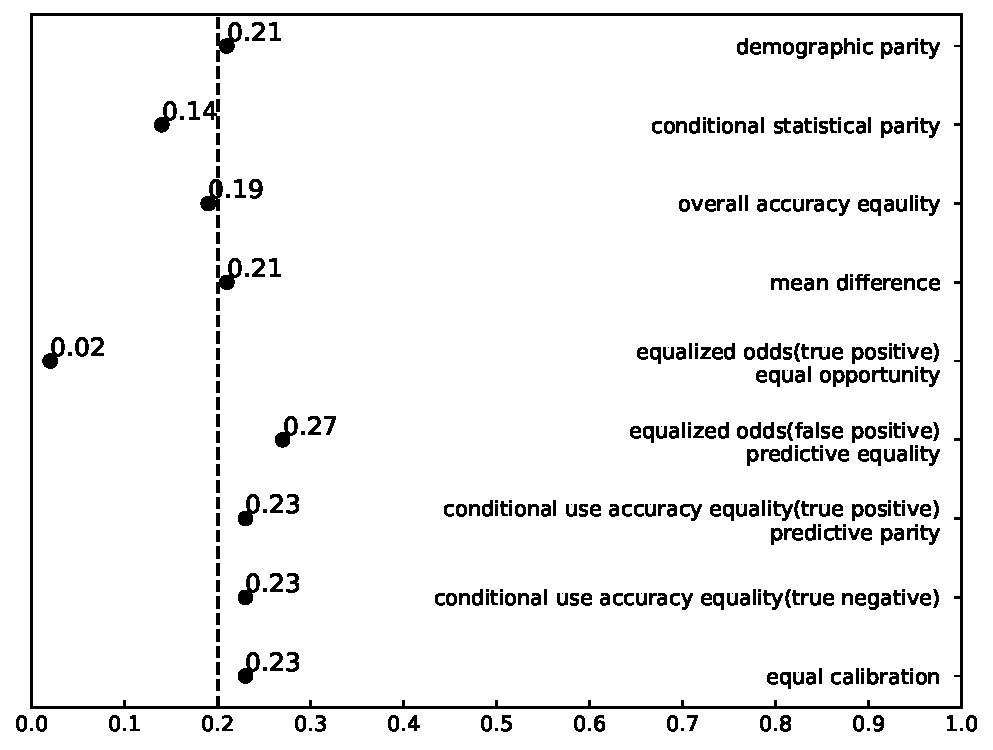
\includegraphics[width=\linewidth]{Non-Asian}
        \subcaption{Privileged Group: Non-Asian}\label{fig:2}
    \end{minipage}
    \hfill
    \begin{minipage}[b]{0.48\linewidth}
        \centering
        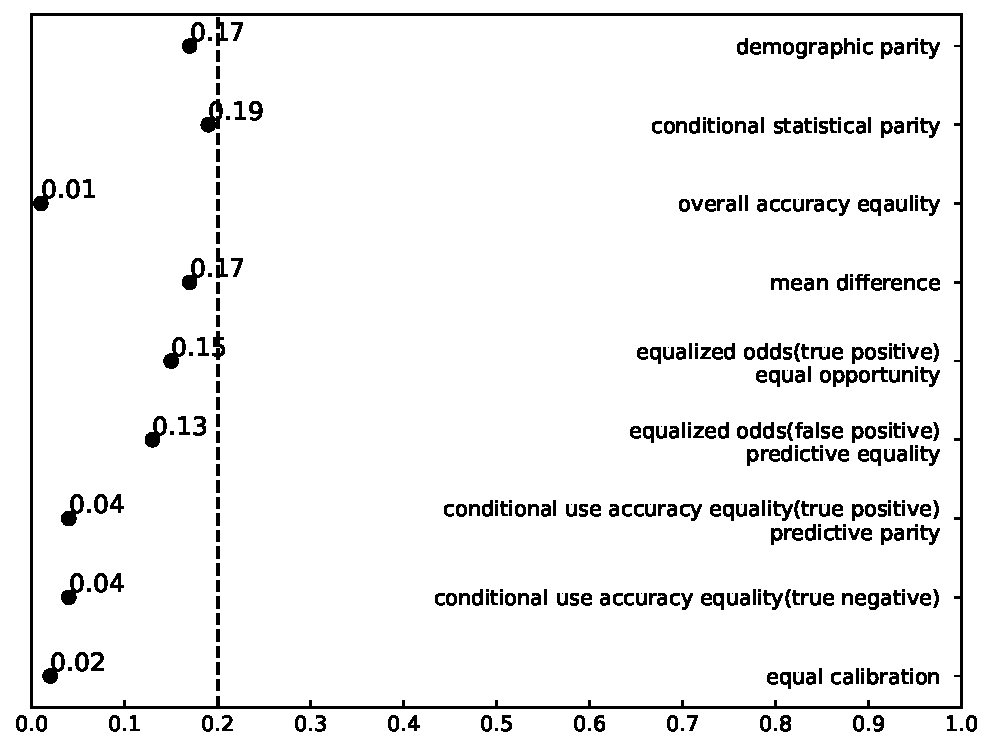
\includegraphics[width=\linewidth]{Non-Caucasian}
        \subcaption{Privileged Group: Non-Caucasian}\label{fig:2}
    \end{minipage}
    \hfill
    \begin{minipage}[b]{0.48\linewidth}
        \centering
        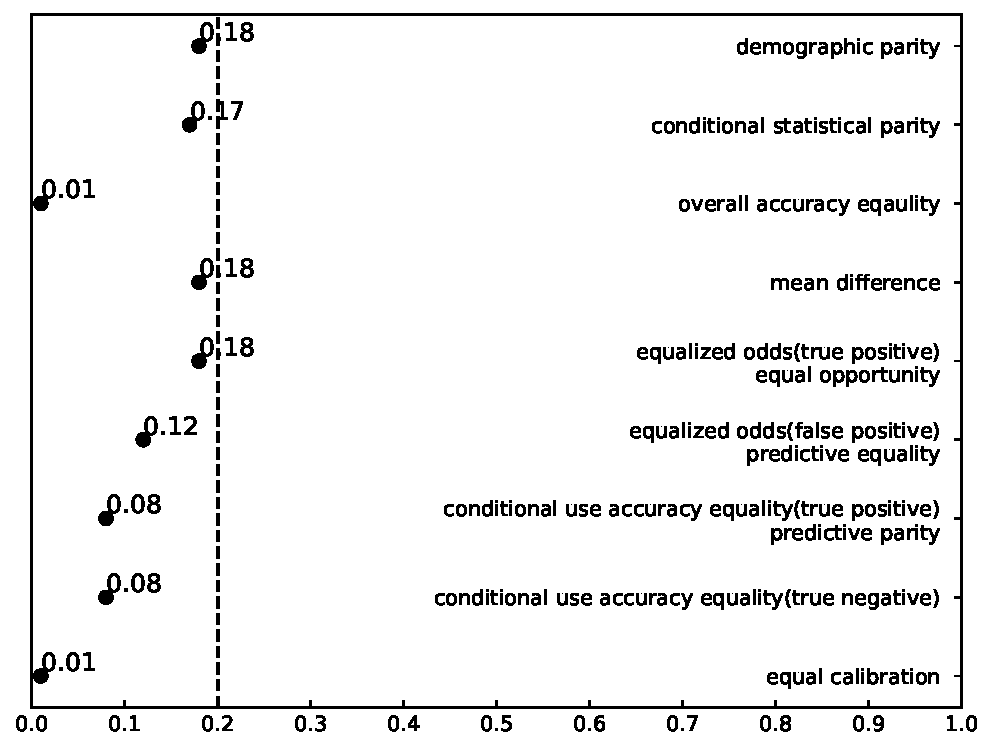
\includegraphics[width=\linewidth]{Non-Hispanic}
        \subcaption{Privileged Group: Non-Hispanic}\label{fig:2}
    \end{minipage}
    \hfill
    \begin{minipage}[b]{0.48\linewidth}
        \centering
        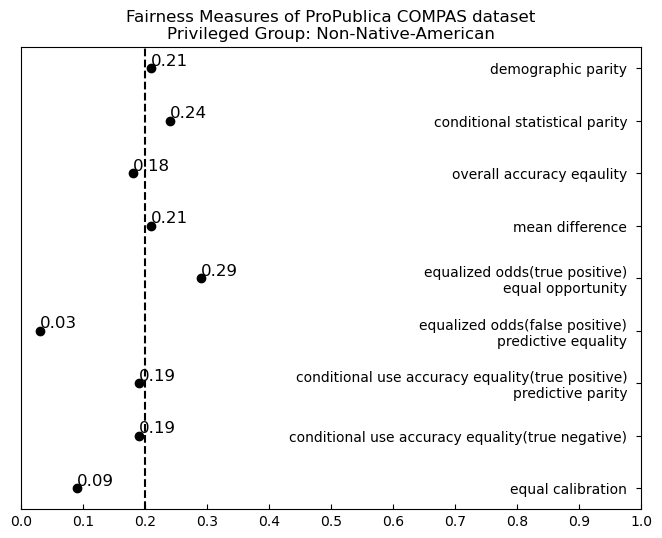
\includegraphics[width=\linewidth]{Non-Native-American}
        \subcaption{Privileged Group: Non-Native-American}\label{fig:2}
    \end{minipage}
    \caption{Fairness Measures of ProPublica COMPAS dataset}
    \label{fig:compas}
\end{figure*}

\bibliographystyle{IEEEtran}
\bibliography{references}

\end{document}




